\documentclass[10pt,landscape]{article}
\usepackage{multicol}
\usepackage{calc}
\usepackage{ifthen}
\usepackage[landscape]{geometry}
\usepackage{graphicx}
\usepackage{amsmath, amssymb, amsthm}
\usepackage{latexsym, marvosym}
\usepackage{pifont}
\usepackage{lscape}
\usepackage{graphicx}
\usepackage{array}
\usepackage{booktabs}
\usepackage[bottom]{footmisc}
\usepackage{tikz}
\usetikzlibrary{shapes}
\usepackage{pdfpages}
\usepackage{wrapfig}
\usepackage{enumitem}
\setlist[description]{leftmargin=0pt}
\usepackage{xfrac}
\usepackage[
            open,
            openlevel=2
            ]{bookmark}
\usepackage{relsize}
\usepackage{rotating}

 \newcommand\independent{\protect\mathpalette{\protect\independenT}{\perp}}
    \def\independenT#1#2{\mathrel{\setbox0\hbox{$#1#2$}%
    \copy0\kern-\wd0\mkern4mu\box0}} 
            
\newcommand{\noin}{\noindent}    
\newcommand{\logit}{\textrm{logit}} 
\newcommand{\var}{\textrm{Var}}
\newcommand{\cov}{\textrm{Cov}} 
\newcommand{\corr}{\textrm{Corr}} 
\newcommand{\N}{\mathcal{N}}
\newcommand{\Bern}{\textrm{Bern}}
\newcommand{\Bin}{\textrm{Bin}}
\newcommand{\Beta}{\textrm{Beta}}
\newcommand{\Gam}{\textrm{Gamma}}
\newcommand{\Expo}{\textrm{Expo}}
\newcommand{\Pois}{\textrm{Pois}}
\newcommand{\Unif}{\textrm{Unif}}
\newcommand{\Geom}{\textrm{Geom}}
\newcommand{\NBin}{\textrm{NBin}}
\newcommand{\Hypergeometric}{\textrm{HGeom}}
\newcommand{\HGeom}{\textrm{HGeom}}
\newcommand{\Mult}{\textrm{Mult}}

\geometry{top=.4in,left=.2in,right=.2in,bottom=.4in}

\pagestyle{empty}
\makeatletter
\renewcommand{\section}{\@startsection{section}{1}{0mm}%
                                {-1ex plus -.5ex minus -.2ex}%
                                {0.5ex plus .2ex}%x
                                {\normalfont\large\bfseries}}
\renewcommand{\subsection}{\@startsection{subsection}{2}{0mm}%
                                {-1explus -.5ex minus -.2ex}%
                                {0.5ex plus .2ex}%
                                {\normalfont\normalsize\bfseries}}
\renewcommand{\subsubsection}{\@startsection{subsubsection}{3}{0mm}%
                                {-1ex plus -.5ex minus -.2ex}%
                                {1ex plus .2ex}%
                                {\normalfont\small\bfseries}}
\makeatother

\setcounter{secnumdepth}{0}

\setlength{\parindent}{0pt}
\setlength{\parskip}{0pt plus 0.5ex}

% -----------------------------------------------------------------------

\usepackage{titlesec}

\titleformat{\section}
{\color{blue}\normalfont\large\bfseries}
{\color{blue}\thesection}{1em}{}
\titleformat{\subsection}
{\color{cyan}\normalfont\normalsize\bfseries}
{\color{cyan}\thesection}{1em}{}
% Comment out the above 5 lines for black and white

\begin{document}

\raggedright
\footnotesize
\begin{multicols*}{3}

% multicol parameters
% These lengths are set only within the two main columns
%\setlength{\columnseprule}{0.25pt}
\setlength{\premulticols}{1pt}
\setlength{\postmulticols}{1pt}
\setlength{\multicolsep}{1pt}
\setlength{\columnsep}{2pt}

%%%%%%%%%%%%%%%%%%%%%%%%%%%%%%%%%%%%
%%% TITLE
%%%%%%%%%%%%%%%%%%%%%%%%%%%%%%%%%%%%

\begin{center}
    {\color{blue} \Large{\textbf{Electromagnetics Cheatsheet}}} \\
   % {\Large{\textbf{Probability Cheatsheet}}} \\
    % comment out line with \color{blue} and uncomment above line for b&w
\end{center}

%%%%%%%%%%%%%%%%%%%%%%%%%%%%%%%%%%%%
%%% ATTRIBUTIONS
%%%%%%%%%%%%%%%%%%%%%%%%%%%%%%%%%%%%

\scriptsize

Compiled by Eigen-$\pi$ (\url{https://www.linkedin.com/in/islamibr29/}).  Licensed under \texttt{\href{http://creativecommons.org/licenses/by-nc-sa/4.0/}{CC BY-NC-SA 4.0}}. Please share comments, suggestions, and errors at \url{http://github.com/islamibr/today_i_learned}.

\begin{center}
    Last Updated \today
\end{center}

%%%%%%%%%%%%%%%%%%%%%%%%%%%%%%%%%%%%
%%% BEGIN CHEATSHEET
%%%%%%%%%%%%%%%%%%%%%%%%%%%%%%%%%%%%

\section{Multi-Variable Calculus}\smallskip \hrule height 2pt \smallskip
    \subsection{Vector Algebra}
    \begin{itemize}
    \item \textbf{Thm 0:} $\vec{A} = <A_i \hat{a}_i, A_j \hat{a}_j, A_k \hat{a}_k>, \ ||\Vec{A}|| = \sqrt{A_i^2 + A_j^2 + A_k^2}$
     \item \textbf{Thm 1:} $||c\Vec{A}|| = |c| \ ||\Vec{A}||$
     \item \textbf{Thm 2:} $\Vec{a} = \frac{\Vec{A}}{||\Vec{A}||}$ a:a is unit vector
     \item \textbf{Thm 3: Dot Product} $ \vec{A} \cdot \vec{B} = A_i B_i + A_j B_j + A_k B_k $
     \item \textbf{Thm 4: Dot Product Properties}
         \begin{tabular}{l|l}
                         $\vec{a} \cdot \vec{b} = (\vec{b} \cdot \vec{a})$ & $(c\vec{a}) \cdot \vec{b} =  \vec{a} \cdot (c\vec{b}) = c (\vec{a} \cdot \vec{b})$ \\
                         $\vec{a} \cdot (\vec{b} + \vec{c}) = \vec{a} \cdot \vec{b} + \vec{a} \cdot \vec{c}$ & $0 \cdot \vec{a} = 0$ \\
                         $(\vec{a} + \vec{b}) \cdot \vec{c} = \vec{a} \cdot \vec{b} + \vec{a} \cdot \vec{c}$ & $\vec{a} \cdot \vec{a} = ||\Vec{A}||^2$ \\
         \end{tabular}
     \item \textbf{Thm 5: Angle} $\vec{a} \cdot \vec{b} = ||\vec{a}|| \ ||\vec{b}|| \ cos \ \theta, \,\, \theta: 0 < \theta < \pi$ 
     \item \textbf{Thm 6: Orthogonality} $\vec{a} \perp
 \vec{b} \Longleftrightarrow \vec{a} \cdot
 \vec{b} = 0$
 \item \textbf{Thm 7: Component (Scalar)} $\text{comp}_{\vec{a}} \vec{b} = 
 ||\vec{b}||  \ cos \ \theta = \frac{\vec{a} \cdot \vec{b}}{||\vec{a}||} $ 
 \item \textbf{Thm 8: Projection (Vector)} $\text{proj}_{\vec{a}} \vec{b} = \text{comp}_{\vec{a}} \vec{b} \cdot \frac{\vec{a}}{||\vec{a}||} = \frac{\vec{a} \cdot \vec{b}}{\vec{a} \cdot \vec{a}} \vec{a}$ 
  \item \textbf{Thm 9: $\perp$ Projection (Vector)} $\text{oproj}_{\vec{a}} \vec{b} = \vec{b} - \text{proj}_{\vec{a}} \vec{b}$ 
  \item \textbf{Thm 10: Cross Product} $ \vec{A} \times \vec{B} = \left\lvert
\begin{matrix}
i & j & k\\
A_i & A_j & A_k \\
B_i & B_j & B_k 
\end{matrix}
\right\rvert$
     \item \textbf{Thm 11: Cross Product Properties}
         \begin{tabular}{l|l}
    $\vec{a} \times \vec{b} = -(\vec{b} \times \vec{a})$ & $(c\vec{a}) \times \vec{b} = \vec{a} \times (c\vec{b}) = c (\vec{a} \times \vec{b})$ \\
    $\vec{a} \times (\vec{b} + \vec{c}) = \vec{a} \times \vec{b} + \vec{a} \times \vec{c}$ & $0 \times \vec{a} = \vec{0}$ \\
    $(\vec{a} + \vec{b}) \times \vec{c} = \vec{a} \times \vec{c} + \vec{b} \times \vec{c}$ & $\vec{a} \times \vec{a} = 0$
\end{tabular}

     \item \textbf{Thm 11: Angle} $\vec{a} \cdot \vec{b} = ||\vec{a}|| \ ||\vec{b}|| \ sin \ \theta, \,\, \theta: 0 < \theta < \pi$ 
     \item \textbf{Thm 12: Parallelity} $\vec{a} \parallel 
 \vec{b} \Longleftrightarrow \vec{a} \times
 \vec{b} = 0$
 \item \textbf{Thm 13:} $\vec{c} = \vec{a} \times
 \vec{b} : \vec{c} \perp \vec{a}, \vec{b}$
 \item \textbf{Thm 14: Area of parallelogram} $||\vec{a} \times
 \vec{b}||$
 \item \textbf{Thm 15: Area of triangle} $\frac{1}{2}||\vec{a} \times
 \vec{b}||$
  \item \textbf{Thm 16: Triple Product (Scalar)} $ \vec{A} \times \vec{B} \cdot \vec{C} = \vec{A} \cdot \vec{B} \times \vec{C} \left\lvert
\begin{matrix}
A_i & A_j & A_k \\
B_i & B_j & B_k \\
C_i & C_j & C_k 
\end{matrix}
\right\rvert$
   \end{itemize}
    \subsection{Vector Geometry}
    \subsubsection{Coordinates}
    \begin{itemize}
        \item Cartesian: $$\vec{A} = <A_x \hat{a}_x, A_y \hat{a}_y, A_z \hat{a}_z>$$ $$-\infty<x,y,z<\infty$$
        \item Cylindrical: $$\vec{A} = <A_{\rho} \hat{a}_{\rho}, A_{\phi} \hat{a}_{\phi}, A_z \hat{a}_z>$$ $$0 \leq \rho < \infty, 0 \leq \phi < 2\pi, -\infty<z<\infty$$
        \item Spherical: $$\vec{A} = <A_r \hat{a}_r, A_{\theta} \hat{a}_{\theta}, A_{\phi} \hat{a}_{\phi}>$$ $$0 \leq r < \infty, 0 \leq \theta < \pi, 0 \leq \phi < 2\pi$$
    \end{itemize}
    \subsubsection{Transformations}
    Cylindrical $\Longleftrightarrow$  Spherical
$$
\begin{bmatrix}
$A_r$\\
$A_\theta$\\
$A_\phi$\\

\end{bmatrix}
=
\begin{bmatrix}
$sin(\theta)$ & 0 & $cos(\theta)$\\
$cos(\theta)$ & 0 & $-sin(\theta)$\\
0 & 1 & 0\\
\end{bmatrix}
\begin{bmatrix}
$A_\rho$\\
$A_\phi$\\
$A_z$\\
\end{bmatrix}
$$

$$
\begin{bmatrix}
$A_\rho$\\
$A_\phi$\\
$A_z$\\
\end{bmatrix}
=
\begin{bmatrix}
$sin(\theta)$ & $cos(\theta)$ & 0\\
0 & 0 & 1\\
$cos(\theta)$$ &  $-sin(\theta)$ & 0\\
\end{bmatrix}
\begin{bmatrix}
$A_r$\\
$A_\theta$\\
$A_\phi$\\
\end{bmatrix}
$$
\begin{center}
    $r= \sqrt{\rho^2 + z^2}$, $\rho = rsin(\theta)$
\\\\\\
$\theta = tan^{-1}(\frac{\rho}{z})$, $z= rcos(\theta)$
\\\\\\
$\phi = \phi$
\end{center}

   Cartesian $\Longleftrightarrow$  Cylindrical
$$
\begin{bmatrix}
$A_\rho$\\
$A_\phi$\\
$A_z$\\
\end{bmatrix}
=
\begin{bmatrix}
$cos(\phi)$ & $sin(\phi)$ & 0\\
$-sin(\phi)$ & $cos(\phi)$ & 0\\
0 $ & 0 & 1\\
\end{bmatrix}
\begin{bmatrix}
$A_x$\\
$A_y$\\
$A_z$\\
\end{bmatrix}
$$

$$
\begin{bmatrix}
$A_x$\\
$A_y$\\
$A_z$\\

\end{bmatrix}
=
\begin{bmatrix}
$cos(\phi)$ & $-sin(\phi)$ & 0\\
$sin(\phi)$ & $cos(\phi)$ & 0\\
0 & 0 & 1\\
\end{bmatrix}
\begin{bmatrix}
$A_\rho$\\
$A_\phi$\\
$A_z$\\
\end{bmatrix}
$$


\begin{center}
    $\rho= \sqrt{x^2 + y^2}$, $x = \rho cos(\theta)$
\\\\\\
$\phi = tan^{-1}(\frac{y}{x})$, $y = \rho sin(\theta)$
\\\\\\
$z = z$
\end{center}

  Cartesian $\Longleftrightarrow$  Spherical
$$
\begin{bmatrix}
$A_r$\\
$A_\theta$\\
$A_\phi$\\

\end{bmatrix}
=
\begin{bmatrix}
$sin(\theta)cos(\phi)$ & $sin(\theta)sin(\phi)$ & $cos(\theta)$\\
$cos(\theta)cos(\phi)$ & $cos(\theta)sin(\phi)$ & $-sin(\theta)$\\
$-sin(\phi)$ & $cos(\phi)$ & 0\\
\end{bmatrix}
\begin{bmatrix}
$A_x$\\
$A_y$\\
$A_z$\\
\end{bmatrix}
$$

$$
\begin{bmatrix}
$A_x$\\
$A_y$\\
$A_z$\\
\end{bmatrix}
=
\begin{bmatrix}
$sin(\theta)cos(\phi)$ & $cos(\theta)cos(\phi)$ & $-sin(\phi)$\\
$sin(\theta)sin(\phi)$ & $cos(\theta)sin(\phi)$ & $cos(\phi)$\\
$cos(\theta)$ & $-sin(\theta)$ & 0\\
\end{bmatrix}
\begin{bmatrix}
$A_r$\\
$A_\theta$\\
$A_\phi$\\
\end{bmatrix}
$$
\begin{center}
    $r= \sqrt{x^2 + y^2 + z^2}$, $x = rsin(\theta)cos(\phi)$
\\\\\\
$\theta = cos^{-1}(\frac{z}{\sqrt{x^2 + y^2 + z^2}})$, $y = rsin(\theta)sin(\phi)$
\\\\\\
$z=rcos(\theta)$, $\phi = tan^{-1} \frac{y}{x}$
\end{center}
Overview \\
\ \begin{minipage}{\linewidth}
            \centering
             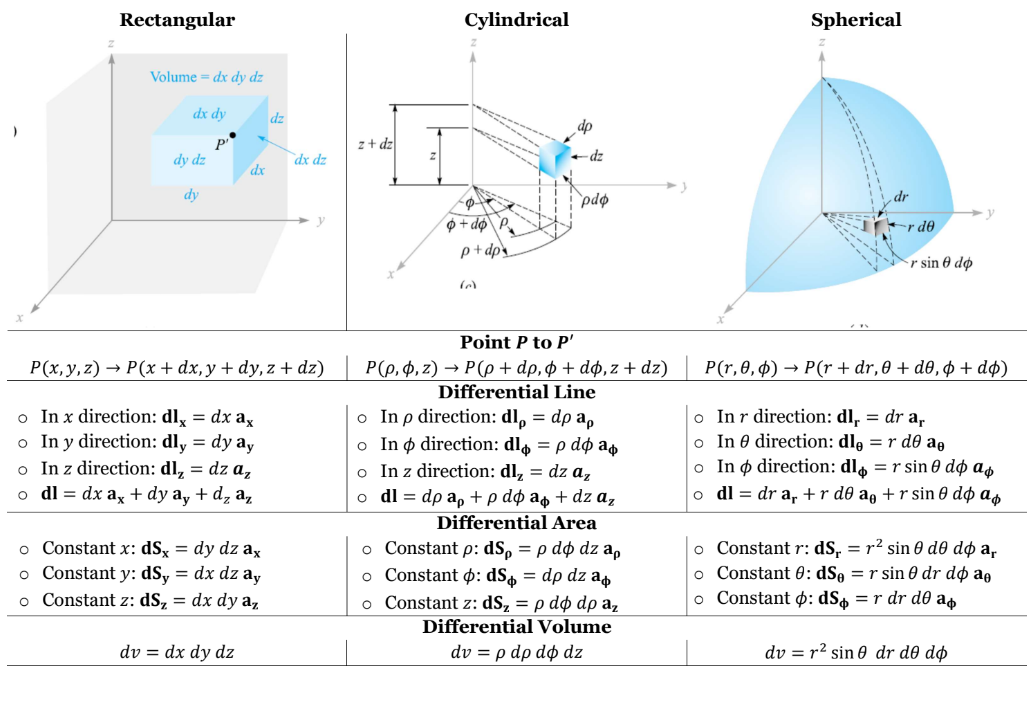
\includegraphics[width=\textwidth]{image.png}
        \end{minipage}
    \subsection{Vector Calculus}
    \begin{itemize}
    \item \textbf{Thm 0: Green} \begin{equation*}
\oint_{\partial D} \vec{F} \cdot d\vec{r} = \iint_{D} \left( \frac{\partial Q}{\partial x} - \frac{\partial P}{\partial y} \right) \,dx\,dy
\end{equation*}
    \item \textbf{Thm 1: Gauss} \begin{equation*}
\iiint_{V} \nabla \cdot \vec{F} \,dV = \oint_{S} \vec{F} \cdot d\vec{S}
\end{equation*}
    \item \textbf{Thm 2: Stokes} \begin{equation*}
\oint_{C} \vec{F} \cdot d\vec{r} = \iint_{S} (\nabla \times \vec{F}) \cdot d\vec{S} \end{equation*} \end{itemize}
     \subsubsection{Nabla} 
      Cartesian:
     \begin{equation*} \nabla = \frac{\partial}{\partial x} \hat{x}+ \frac{\partial}{\partial y} \hat{y}+ \frac{\partial}{\partial z} \hat{z}
\end{equation*}
Cylindrical:
\begin{equation*}
\nabla = \frac{\partial}{\partial \rho} \hat{\rho}+ \frac{1}{\rho} \frac{\partial}{\partial \phi} \hat{\phi} + \frac{\partial}{\partial z}\hat{z}
\end{equation*}

Spherical:

\begin{equation*}
\nabla =  \frac{\partial}{\partial r}\hat{r} + \frac{1}{r} \frac{\partial}{\partial \theta} \hat{\theta}+ \frac{1}{r \sin(\theta)} \frac{\partial} {\partial \phi}\hat{\phi}
\end{equation*}

    \subsubsection{Div}
    Cartesian:
    $$\nabla \cdot \vec{D} = \frac{\partial D_x}{\partial x} + \frac{\partial D_y}{\partial y} + \frac{\partial D_z}{\partial z}$$
    Cylindrical:
    $$\nabla  \cdot \vec{D} = \frac{1}{\rho}\frac{\partial \rho D_{\rho}}{\partial \rho} +\frac{1}{\rho} \frac{\partial D_{\phi}}{\partial \phi} + \frac{\partial D_z}{\partial z}$$
    Spherical:
     $$\nabla \cdot \vec{D} = \frac{1}{r^2}\frac{\partial r^2 D_{r}}{\partial r} +\frac{1}{rsin\theta} \frac{\partial sin\theta D_{\theta}}{\partial \theta} + \frac{1}{rsin\theta} \frac{\partial D_{\phi}}{\partial \phi}$$
     \subsubsection{Curl}
    Cartesian:
         $$\nabla \times \vec{H} = \left\lvert
\begin{matrix}
a_x & a_y & a_z \\
\frac{\partial}{\partial x} & \frac{\partial}{\partial y} & \frac{\partial}{\partial z} \\
H_x & H_y & H_z 
\end{matrix}
\right\rvert$$

    Cylindrical:
$$\nabla \times \vec{H} = \frac{1}{\rho}\left\lvert
\begin{matrix}
a_{\phi} & a_{\phi} & a_z \\
\frac{\partial}{\partial \rho} & \frac{\partial}{\partial \phi} & \frac{\partial}{\partial z} \\
H_{\rho} & \rho H_{\phi} & H_{z} 
\end{matrix}
\right\rvert$$

    Spherical:
   $$\nabla \times \vec{H} = \frac{1}{r^2sin\theta}\left\lvert
\begin{matrix}
a_{r} & a_{\theta} & a_z \\
\frac{\partial}{\partial r} & \frac{\partial}{\partial \theta} & \frac{\partial}{\partial \phi} \\
H_{\rho} & r H_{\theta} & r sin\theta H_{\phi} 
\end{matrix}
\right\rvert$$

\subsubsection{Notes}
\begin{center}
    \begin{tabular}{l|l}
    \centering
    $\nabla \cdot D = 0$ & $\nabla \times H = 0$ \\
    Divergent-free & Curl-free \\
    Source-free & Irrational \\
    Solenoid & Conservative
\end{tabular}
\end{center}

\begin{itemize}
    \item Gradient is Vector indicates the encreasing direction.
    \item Div is Scalar indicates sources (+ve) and sinks (-ve).
    \item Curl is Vector indicates rotation ccw (+ve) and cw (-ve). 
    \item Div of Curl = 0, Curl of Grad = 0, Div of Grad = Laplace.
    \item Closed integral doesn't depends on path in case of curl-free.
\end{itemize}
\newpage
\section{Static Electromagnetism} \smallskip \hrule height 2pt \smallskip
\subsection{Maxwell Equations}
\begin{center}
    \begin{tabular}{c|c|c}
         & \textbf{Integral Form} & \textbf{Point Form} \\
        \hline
        \textbf{Kirchhoff's Voltage Law} & $\oint \vec{E} \cdot d\vec{L} = 0$ & $\nabla \times \vec{E} = 0$ \\
        \textbf{Ampere's Current Law} & $\oint \vec{H} \cdot d\vec{L} = \int \vec{J} \cdot d\vec{S} = I_{enc}$ & $\nabla \times \vec{H} = J$ \\
        \textbf{Gauss's Law for E-Field} & $\oint \vec{D} \cdot d\vec{S} = \int \rho d{V}$ & $\nabla \cdot \vec{D} = \rho_v$ \\
        \textbf{Gauss's Law for H-Field} & $\oint \vec{B} \cdot d\vec{S} = 0 $&  $\nabla \cdot \vec{B} = 0$ \\
        
    \end{tabular}
\end{center}

\subsection{Analogy Between Electric and Magnetic}
   \begin{center}
    \begin{tabular}{c|c}
        \textbf{Electric Field Intensity} $\vec{E}$ [$\frac{V}{m}$] & \textbf{Magnetic Field Intensity} $\vec{H}$ [$\frac{A}{m}$] \\
        \hline \\
        Permittivity $\epsilon = \epsilon_0 \epsilon_r$ [$\frac{F}{m}$] & Permeability $\mu = \mu_0 \mu_r$ [$\frac{H}{m}$] \\ \\
        Coulomb's Law & Biot-Savart Law  \\ $dE = \frac{dQ}{4\pi \epsilon R^2} \vec{a}_r \Longleftrightarrow E = \int \frac{dQ}{4\pi \epsilon R^2} \vec{a}_r$ & $dH = \frac{Id\vec{L} \times \vec{a}_r}{4\pi \epsilon R^2} \Longleftrightarrow H = \int \frac{Id\vec{L} \times \vec{a}_r}{4\pi \epsilon R^2}$ \\ \\
        Kirchhoff Voltage Law & Ampere Current Law\\
        $\oint \vec{E} \cdot d\vec{L} = 0$ & $ \oint \vec{H} \cdot d\vec{L} = I_{enc} $  \\ 
        $\nabla \times \vec{E} = 0$ & $\nabla \times \vec{H} = J$ \\ \\
        Electric Flux Density & Magnetic Flux Density \\
        $\vec{D} = \epsilon \vec{E} $ [$\frac{C}{m^2}$] &  $\vec{B} = \mu \vec{H} $ [$\frac{\text{Wb}}{m^2}$] \\ \\
        Electric Flux Lines & Magnetic Flux Lines \\
        $\psi =  \oint \vec{D} \cdot d\vec{S} \ [C]$ & $\phi =  \int_S \vec{B} \cdot d\vec{S} \ [\text{Wb}]$ \\ \\
        Gauss Law for E-Field & Gauss Law for H-Field \\ 
        $\oint \vec{D} \cdot d\vec{S} = Q_{enc}$ & $\oint \vec{B} \cdot d\vec{S} = 0$ \\
        $\nabla \cdot \vec{D} = \rho_v$ & $\nabla \cdot \vec{B} = 0$ \\ \\
        Stored Electric Energy & Stored Magnetic Energy \\
        $W_E = \frac{1}{2} \int \vec{D} \cdot \vec{E} \, dv$ & $W_E = \frac{1}{2} \int \vec{B} \cdot \vec{H} \, dv$ \\
        $\vec{D} \cdot \vec{E} = \epsilon E^2 = \frac{D^2}{\epsilon}$ & $\vec{B} \cdot \vec{H} = \mu H^2 = \frac{B^2}{\mu}$ \\ 
         & $W_E = \int \vec{B} \cdot d\vec{H}$ \\ \\
        Uniform E-Flux Lines & Uniform H-Flux Lines \\
        $\psi = \vec{D} \cdot \vec{A} = Q_{enc}$ & $\psi = \vec{B} \cdot \vec{A}$ \\ \\
        Electric Force & Magnetic Force \\
        $\arc{F} = q\arc{E}$ & $\arc{F} = q(\arc{v} \times \arc{B})$ \\ \\
        
        
        
    \end{tabular}
\end{center}

\subsection{All Differential Elements}
\begin{itemize}
    \item \textbf{Electric Field}
\[
dE = 
\begin{cases}
    \frac{\rho_L dl}{4 \pi R^2 \epsilon} \vec{a}_r & \text{Line}, \\ \\
    \frac{\rho_S dS}{4 \pi R^2 \epsilon} \vec{a}_r & \text{Surface}, \\ \\
    \frac{\rho_V dV}{4 \pi R^2 \epsilon} \vec{a}_r & \text{Volume}.
\end{cases}
\]
    \item \textbf{Electric Potential}
    \[
dV = 
\begin{cases}
    \frac{\rho_L dl}{4 \pi R \epsilon} \vec{a}_r & \text{Line}, \\ \\
    \frac{\rho_S dS}{4 \pi R \epsilon} \vec{a}_r & \text{Surface}, \\ \\
    \frac{\rho_V dV}{4 \pi R \epsilon} \vec{a}_r & \text{Volume}.
\end{cases}
\]

\item \textbf{Magnetic Field}
$$dH = \frac{Id\vec{L} \times \vec{a}_r}{4\pi R^2}$$
\end{itemize}
\subsection{Analogy Between Capacitance and Inductor}
   \begin{center}
    \begin{tabular}{c|c}
        \textbf{Capacitance}  & \textbf{Inductor}  \\
        \hline \\
        Capacitance & Inductance \\
        $C=\frac{Q}{V} = \frac{\epsilon A}{l}$ & $L=\frac{N\Phi}{I} = \frac{NBA}{I}$  \\ \\ Relative Permittivity &  Relative Permeability \\
        $\epsilon_r = \frac{C}{C_o} = \frac{Q}{Q_o}$ & $\mu_r = \frac{L}{L_o} = \frac{B}{B_o}$\\ \\
        Electric Dipole Moment & Magnetic Dipole Moment  \\ 
        $\vec{p} = Q\vec{x}$ & $\vec{m} = IA\vec{a}_n$ \\ \\
        Polarization & Magnetization \\
        $\vec{P} = \epsilon_o (\epsilon_r - 1) \vec{E} $ &  $\vec{M} = (\mu_r - 1) \vec{H}$ \\ 
        $\vec{P} = \frac{\epsilon_r-1}{\epsilon_r} \vec{D} = \frac{n \vec{p}}{V}$ &  $\vec{M} = \frac{I_m}{l}$ \\ \\
        Electric Susceptibility  & Magnetic Susceptibility \\
        $\chi_e =  \epsilon_r - 1$ & $\chi_m =  \mu_r - 1$ \\ \\
        Energy Stored in Capacitor & Energy Stored in Inductor \\ 
        $W_E = \frac{1}{2} CV^2$ & $W_H = \frac{1}{2} LI^2$ \\ 
        $\nabla \cdot \vec{D} = \rho_v$ & $\nabla \cdot \vec{B} = 0$ \\ \\
        DC Electric Field Intensity & DC Magnetic Field Intensity \\
        $E = \frac{V}{l}$ & $H = \frac{NI}{l} = \frac{I_c}{l}$ \\ \\
        Electric Boundary Conditions & Magnetic Boundary Conditions \\
        Conductors & - \\
        $E_t = 0, D_N = \epsilon E_N = \rho_s : E_N = - \nabla V $ & - \\ \\
        Dielectric  & - \\
        $E_{t1} = E_{t2}, D_{n1} = D_{n2}$ & - \\ $ \epsilon_1 E_{n1} = \epsilon_2 E_{n2} $ & - \\ $ \frac{tan\theta_1}{tan\theta_2} = \frac{\epsilon_1}{\epsilon_2}$ & - \\ \\
        
    \end{tabular}
\end{center}

\subsection{Common Formulas}
\begin{itemize}
    \item Electric Field due Point Charge 
    $$ \vec{E} = \frac{Q}{4\pi \epsilon R^2} \vec{a}_R$$
     \item Electric Potential due Point Charge 
    $$ V = \frac{Q}{4\pi \epsilon R}$$
    \item Electric Field due Infinite Line Charge
    $$ \vec{E} = \frac{\rho_l}{2\pi \epsilon \rho} \vec{a}_{\rho}$$
    \item Electric Field due  Infinite Plane Charge
    $$ \vec{E} = \frac{\rho_s}{2\epsilon}  \vec{a}_{n}$$
     \item Magnetic Field due Infinite Line Current
    $$ \vec{H} = \frac{I}{2\pi \rho} \vec{a}_{\phi}$$
\end{itemize}

\subsection{Other Formulas}
\begin{itemize}
    \item Charge \[
Q = 
\begin{cases}
   \int \rho_L dL & \text{Line}, \\ \\
    \int \rho_S dS & \text{Surface}, \\ \\
     \int \rho_V dV & \text{Volume}.
\end{cases}
\]
    \item Electric Flux Density $\vec{D} = \frac{d\psi}{ds} \vec{a}_{\psi}$
     \item Electric Work $W = - Q \int \vec{E} \cdot d\vec{L} = QV$
     \item Electric Potential $V_{AB} = V_A - V_B = - \int_B^A \vec{E} \cdot d\vec{L}$
     \item Electric Potential with Field $\vec{E} = -\nabla V$
     \item Poisson Equation $\nabla^2 V = \frac{- \rho}{\epsilon}$
     \item Laplace Equation $\nabla^2 V = 0$
     \item Electric Energy $U = \frac{1}{2} \sum QV =\frac{1}{2} \int \rho_v V dv$ 
     \item Force in Conductors 
    $$ \vec{F} = m\vec{a} = - e \vec{E}, \vec{a} = \frac{\vec{v}_d}{\tau}, \vec{v}_d = - \frac{e\tau}{m} \vec{E} = -\mu_e \vec{E}$$
    \item  Current and Current Density $\vec{J} = \sigma \vec{E} = \rho_e \vec{v}_d = -\mu_e \rho_e \vec{E}$ \\ 
    \item  Current $I = \int \vec{J} \cdot d\vec{S}$
    \item $n (\text{electron/m}^3) = \frac{\rho (\text{Density}) N_A (\text{Avogadro’s number})}{M_g \text{ (atomic mass)}}$
    \item \text{Electron Density}  $\rho_e = en$
    \item Ohm's Law $R = \frac{V}{I} = \frac{\int \vec{E} \cdot d\vec{L}}{\int \sigma \vec{E} \cdot d\vec{S}}$
    \item Continuity of Current $\nabla \cdot \vec{J} = - \frac{\partial \rho_v}{\partial t} \Longleftrightarrow \oint \vec{J} \cdot d\vec{S} = - \frac{dQ}{dt}$
    \item Current Elements due to Magnet $$F = -I \oint \vec{B} \times d\vec{L}, F= I (\vec{L} \times \vec{B}) \ \ \text{for straight conductor}$$
    \item Torque due to Magnet $\vec{T} = \vec{R} \times \vec{F} = \vec{R} \times (I (\vec{L} \times \vec{B}))$
    \item Torque due to Magnetic dipole $\vec{T} = \vec{m} \times \vec{B}$
    \item Current due to electron spin $I = e \frac{\omega}{2\pi}$
    \item Faraday's Law $V = NA \frac{dB}{dt}$
\end{itemize}

\subsection{Serious Notes}
\begin{itemize}
    \item \textbf{Ch.1}
    \begin{itemize}
        \item Convert from any system to Cartesian then covert back if you have points and need vector between.
        \item For Cartesian Indicates by three planes. \item For Cylindrical Indicates by two planes and Cylinder. \item For Spherical Indicates by Sphere, Convex and plane.
        \item Magnitude is the same in all systems.
    \end{itemize}
    \item \textbf{Ch.2}
    \begin{itemize}
                \item $\int \frac{dx}{(a^2 + x^2)^{3/2}} = \frac{x}{a^2\sqrt{x^2 + a^2}}$
                \item $\int \frac{x dx}{(a^2 + x^2)^{3/2}} = \frac{-1}{\sqrt{x^2 + a^2}}$
                \item $\int \frac{dx}{a^2 + x^2} = \frac{1}{a}tan^{-1}(\frac{x}{a})$
    \end{itemize}
    \item \textbf{Ch.3}
    \begin{itemize}
                \item Length with D is changeable anywhere but isn't for Q.
                \item Flux lines = Q [$C$]
                \item Flux density $[C/m, C/m^2 C/m^3]$
    \end{itemize}
    \item \textbf{Ch.4}
    \begin{itemize}
                \item Potential and Work are independent of path.
                \item $\nabla V = -\vec{E}$ is normal to equipotential surface and $V$ is max when $d\vec{L}$ in the same diraction.
                \item Work is done by system if it is (-ve).
                \item Workdone for putting first charge = 0
    \end{itemize}
    \item \textbf{Ch.5}
    \begin{itemize}
                \item Charge on the surface of conductor is equal any where and no charge inside so $\vec{E}_{\title{inside}} = 0$.
                \item Charging the inside charging the surface by negative Q.
    \end{itemize}
    \item \textbf{Ch.6}
    \begin{itemize}
                \item After adding dielectric material we get:
                $$ Q = Q_o + Q_p $$
                $$ \vec{D} = \vec{D}_o + \vec{P} $$
                $$ \epsilon_o \epsilon_r \vec{E} = \epsilon_o \vec{E}_o + \vec{P} $$
                $$ \vec{P} = \epsilon_o (\epsilon_r - 1)  \vec{E}  $$
                \item Dielectric have charges on surface and inside.
                \item Dipole direction form (-ve) to (+ve).
                \item Q' = Q after removing the dielectric and battery.
                \item Electric Field inside dielectric $<$ External Field.
    \end{itemize}
    \item \textbf{Ch.7}
    \begin{itemize}
                \item After adding dielectric material we get:
                $$ \phi = \phi_o + \phi_m $$
                $$ \vec{B} = \vec{B}_o + \vec{B}_m $$
                $$ \mu_o \mu_r \vec{H} = \mu_o \vec{H}_o + \mu_o \vec{M} $$
                $$ \vec{M} = (\mu_r - 1)  \vec{H} $$
                \item The magnetization forms surface current.
                \item Magnetization direction is normal.
                \item Cylindrical $ \vec{r} \times \vec{\phi} = \vec{z}, \vec{\phi} \times \vec{z} = \vec{r}, \vec{z} \times \vec{r} = \vec{\phi}$
                \item Spherical $ \vec{r} \times \vec{\theta} = \vec{\phi}, \vec{\theta} \times \vec{\phi} = \vec{r}, \vec{\phi} \times \vec{r} = \vec{\theta}$
                \item Toroid Coil is same as Normal Coil as $l_{\text{coil}} = 2 \pi r_{\text{toroid}}$
                \item No monopole existence.\
                \item Magnetic Field rotate the electrons in circular motion between electric field accelerate/decelerate electrons.
                \item Workdone by Magnetic Field on proton $> 0$
                \item As $\nabla \cdot \vec{B} = 0$, So B has no sink/start or source/end and As $\nabla \times \vec{E} = 0$ So, E has no rotations.
    \end{itemize}
\end{itemize}

\end{multicols*}
\end{document}